\chapter{Soluzione Proposta}
\label{chap:Cap1}
L'idea del progetto nasce dalla volontà di fornire un'integrazione degli acceleratori, in un ambiente cloud tramite l'architettura OpenStack. L'intenzione è  quella di avere presenti in un'interfaccia web la possibilità di prenotare risorse cloud, tra le quali sono presenti le FPGA, le risorse saranno usabili sia per scopi didattici sia per ricerca.
\begin{figure}[h]
\centering
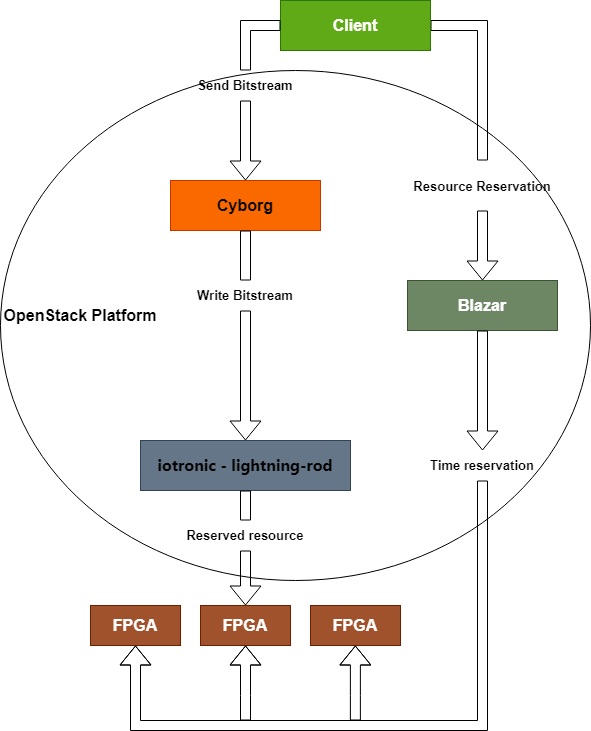
\includegraphics[width=0.45\textwidth]{images/Stack1.png}
\caption{Stack dell'architettura}
\end{figure}\clearpage
Un esempio applicativo potrebbe essere un laboratorio virtuale, dove ogni utente finale, professori, studenti o utenti privati, hanno accesso ad un'infrastruttura che presenta molte risorse cloud tra cui le FPGA, sulle quali è possibile effettuare il caricamento del proprio bitstream precedentemente prodotto.\\
Quest'architettura potrebbe esser vista come un sistema di prenotazione delle risorse per il Cloud Computing, portando ad un incremento di performance rispetto alle strutture classiche grazie all'uso delle FPGA. Tramite la loro riprogrammazione si garantisce una maggior flessibilità, una maggior potenza computazionale e soprattutto la divisione in regioni, che permette la possibilità di ospitare più acceleratori in un singolo device in modo da avere più risorse virtuali disponibili nel cloud, ma con lo stesso numero di board.\\
Le varie fasi del processo verranno effettuate da diversi servizi presenti nella piattaforma \textit{OpenStack}.\\
Il servizio che orchestra le risorse sarà \textit{Blazar}, come spiegato nella sotto sezione \ref{Blazar}, il quale permette la \textit{Resource Reservation} e tramite un altro servizio che effettua il WebServer sarà possibile invocare le API che permettono la reservation.
\begin{figure}[h]
\centering
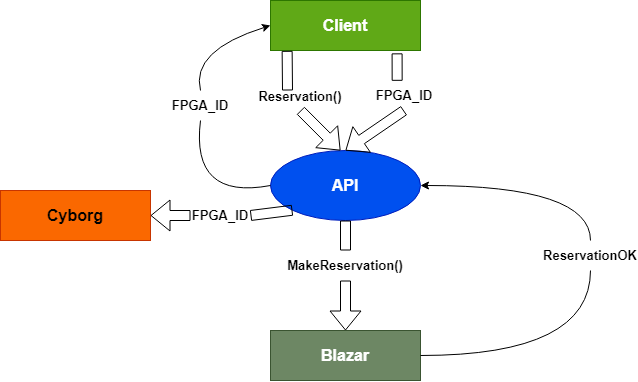
\includegraphics[width=0.4\textwidth]{images/Arch1.png}
\caption{Diagramma che rappresenta le fasi di reservation}
\end{figure}\\
Una volta avvenuta l'effettiva prenotazione, l'utente finale utilizza il servizio \textit{Cyborg},  che gestisce il ciclo di vita degli acceleratori e tramite la sua integrazione con \textit{Nova}, garantisce la virtualizzazione delle FPGA rendendo disponibile la gestione da parte dell'utente dei nodi da quest'ultimo riservati. Al fine di creare il punto di contatto tra il cloud e i dispositivi IoT verranno usati in simbiosi IoTronic e Lightning-rod, integrabili nella piattaforma OpenStack e quindi interfacciabili tramite le API agli altri servizi già presenti nel sistema. Per come sono stati definiti IoTronic sarà l'agente che verrà eseguito lato cloud, mentre Lightning-rod sarà l'agente che verrà eseguito lato FPGA SoC. IoTronic e Lightning-rod saranno connessi tra di loro tramite una connessione \textit{WAMP} in modo da garantire il trasferimento del file binario e l'esecuzione di tutti gli script necessari alla riprogrammazione.
\begin{figure}[h]
\centering
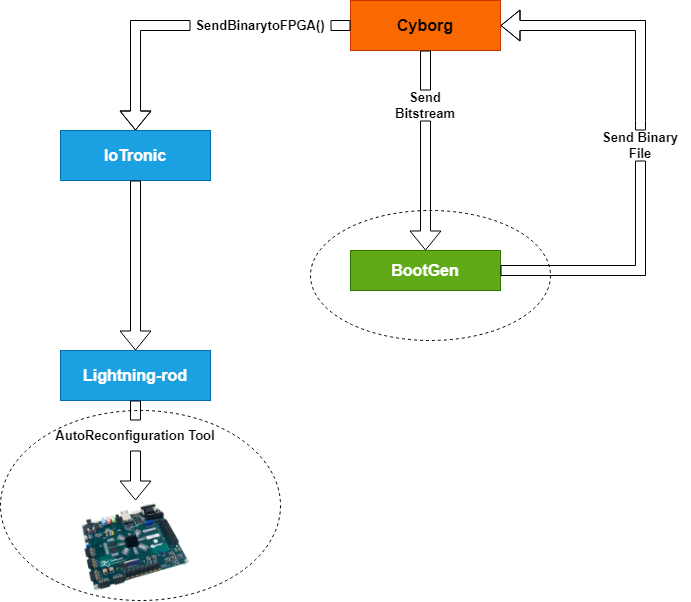
\includegraphics[width=0.6\textwidth]{images/Arch.png}
\caption{Diagramma che rappresenta le fasi post upload del bitstream}
\end{figure}\\
La scelta di fornire il bitstream e quindi aggiungere un livello di complessità in più,  permette di effettuare un'analisi più accurata della validità del bitstream per l'architettura prenotata tramite la sua decodifica. Il bitstream contiene informazioni riguardo la data di creazione, l'architettura e la dimensione. Questo controllo permette di limitare gli errori che un utente novizio può commettere riservando delle risorse non compatibili alla sua architettura.\\
Tutto il sistema è gestito dalle API di OpenStack, il quale garantisce questa integrazione tra servizi diversi tra di loro, rendendo il tutto trasparente all'utente finale.\\
In questa tesi verrà trattato il processo di automatizzazione per la generazione del file binario e per la riprogrammazione automatica tramite Lightning-rod.
 


